%%%%%%%%%%%%%%%%%%%%%%%%%%%%%%%%%%%%%%%%%%%%%%%%%%%%%%%%%%%%%%%%%%%%%%%%%%%%%%%%%%%%%%%
%
%   Web application                   
%
%%
%%%%%%%%%%%%%%%%%%%%%%%%%%%%%%%%%%%%%%%%%%%%%%%%%%%%%%%%%%%%%%%%%%%%%%%%%%%%%%%%%%%%%
\section{Web Application}
% On a l'architecture suivante :
% Client Web <-> Serveur Web <-> Base de données

The main purpose of the computer science team was to develop a sustainable web application that could enable the user to foresee his energy consumption and handle it.  This section introduces the design of this app in wich a database, a server and a web client are the main components. It was built using the following architecture:

    \begin{figure}[!h] % montrer sur le schéma que le server ne fait que servir les données et que c'est le client qui doit en faire le traitement : http://fr.slideshare.net/scothis/aoa-mwa slide 19
        \centering
        \begin{tikzpicture}[node distance=1.5cm]
    
        %%%%% verticale 
        % \node (client) [process, fill=green!10] {Client};
        % \node (server) [process, below of=client, fill=red!10] {Server};
        % \node (db) [process, below of=server, fill=blue!10] {Database};

        % \draw [arrow] (client) -- (server);
        % \draw [arrow] (server) -- (client);
        % \draw [arrow] (server) -- (db);
        % \draw [arrow] (db) -- (server);
        
        %%%% horizontale
        \node (client) [process, fill=green!10] {Client};
        \node (server) [process, right of=client, xshift=3cm, fill=red!10] {Server};
        \node (db) [process, right of=server, xshift=3cm , fill=blue!10] {Database};

        \draw [arrow] (client) -- (server);
        \draw [arrow] (server) -- (client);
        \draw [arrow] (server) -- (db);
        \draw [arrow] (db) -- (server);
        \end{tikzpicture}
    \end{figure}
% 
% le but de l'appli : pouvoir gérer sa conso et sa facture
% le but de l'equipe de dev : maintenable et reprise.


%%%%%%%%%%%%%%%%%%%%%%%%%%%%%
%       Server              %
%%%%%%%%%%%%%%%%%%%%%%%%%%%%%
%%%%%%%%%%%%%%%%%%%%%%%%%%%%%%%%%%%%%%%%%%%%%%%%%
%       Server                                  %
%                                               %
%%%%%%%%%%%%%%%%%%%%%%%%%%%%%%%%%%%%%%%%%%%%%%%%%
\subsection{Server \& Database}

% doit tourner sur Raspberry Pi 
%   -> serveur léger -> lighttpd
%   -> db -> sqlite
%
%   php
%   ¿ interface C/C++ pour le signal ?
%%
%%%
%%
%
% la partie Serveur Web + Base de données étant deployée sur la rasberrypi qui a peu de ressources, les technos utilisées dans cette partie doivent consommer peu de ressources d'où le choix de SQLite et Lighttpd
%
% Ensuite faut dire en quoi SQLITE et Lighttpd sont légers, par exemple SQLite fonctionne sans serveur mais juste en lecture écriture de fichiers, et chercher pour lighttpd des arguments aussi.
%
% Ensuite vu que le serveur ne fait que servir les données, il faut que toute la génération des vues se fasse du coté client d'où le choix d'AngularJS ...

The web server and the database are the links between the signal processing algorithms and the web application. For this project, they are deployed on the single-board computer \textit{Raspberry Pi}. Since it has low ressources, the technologies used for the server and the database have to consume few resources. That is why SQLite and Lighttpd were chosen respectively for the database and the server.

\subsubsection{Database}

    % en quoi sqlite est léger
    %   http://www.sqlite.org/limits.html
    %   http://sqlite.org/mostdeployed.html
    % simplicité : il n'y a aucune manipulation à faire, le fichier sqlite est créé automatiquement à la volée, toute la base est stockée dans un fichier unique qu'il est facile d'échanger. 
    % http://en.wikipedia.org/wiki/SQLite
    \paragraph{SQLite Database}
    
    SQLite is a standalone relational database management system. In contrast to other database management systems, it is not implemented as a separate process that a client program running in another process accesses. Rather, it is part of the using program. SQLite is a popular choice as embedded database for local/client storage in application software such as web browsers. It is one of the most widely deployed database engine, as it is used today by several widespread browsers, operating systems, and embedded systems, among others. 
    
    
    % Structure de la base
    % description des tables etc..
    \paragraph{Structure}
    
    This paragraph introduces the different tables of the database. It has been built to be easily reshaped depending on the research results, and also to deal with big data issues. % ce n'est pas vraiment big data...
    
    \begin{itemize} % ¿ lists ou manage ?
    \item Sensors identification: lists all sensors connected to the system
    \item Locations: lists all sensor locations
    \item Data types: lists the different data types handled by the system
    \item Sensors values: lists the different sensors values recorded over time
    \item Devices types identification: lists the different device types identificated
    \item Devices status: lists all device statuses
    \item User: lists all user information
    \end{itemize}
    
    % ajouter schéma conceptuel de la base.
    
\subsubsection{Server}

    % le serveur ne fait que servir les données
    With the chosen architecture, the web server only sends the data to the client dealing with their processing.
    
    % en quoi lightpd est léger
    % cf references de http://en.wikipedia.org/wiki/Lighttpd
    \paragraph{Lighttpd Server}
    Lighttpd is a secure, fast, compliant, and flexible web server that has been optimized for high-performance environments. It has a very low memory footprint compared to other web servers and takes care of cpu-load.








%%%%%%%%%%%%%%%%%%%%%%%%%%%%%
%       Client              %
%%%%%%%%%%%%%%%%%%%%%%%%%%%%%
%%%%%%%%%%%%%%%%%%%%%%%%%%%%%%%%%%%%%%%%%%%%%%%%%
%       Client                                  %
%                                               %
%%%%%%%%%%%%%%%%%%%%%%%%%%%%%%%%%%%%%%%%%%%%%%%%%
\subsection{Client} % Interface Client
\begin{figure}[H]
\centering
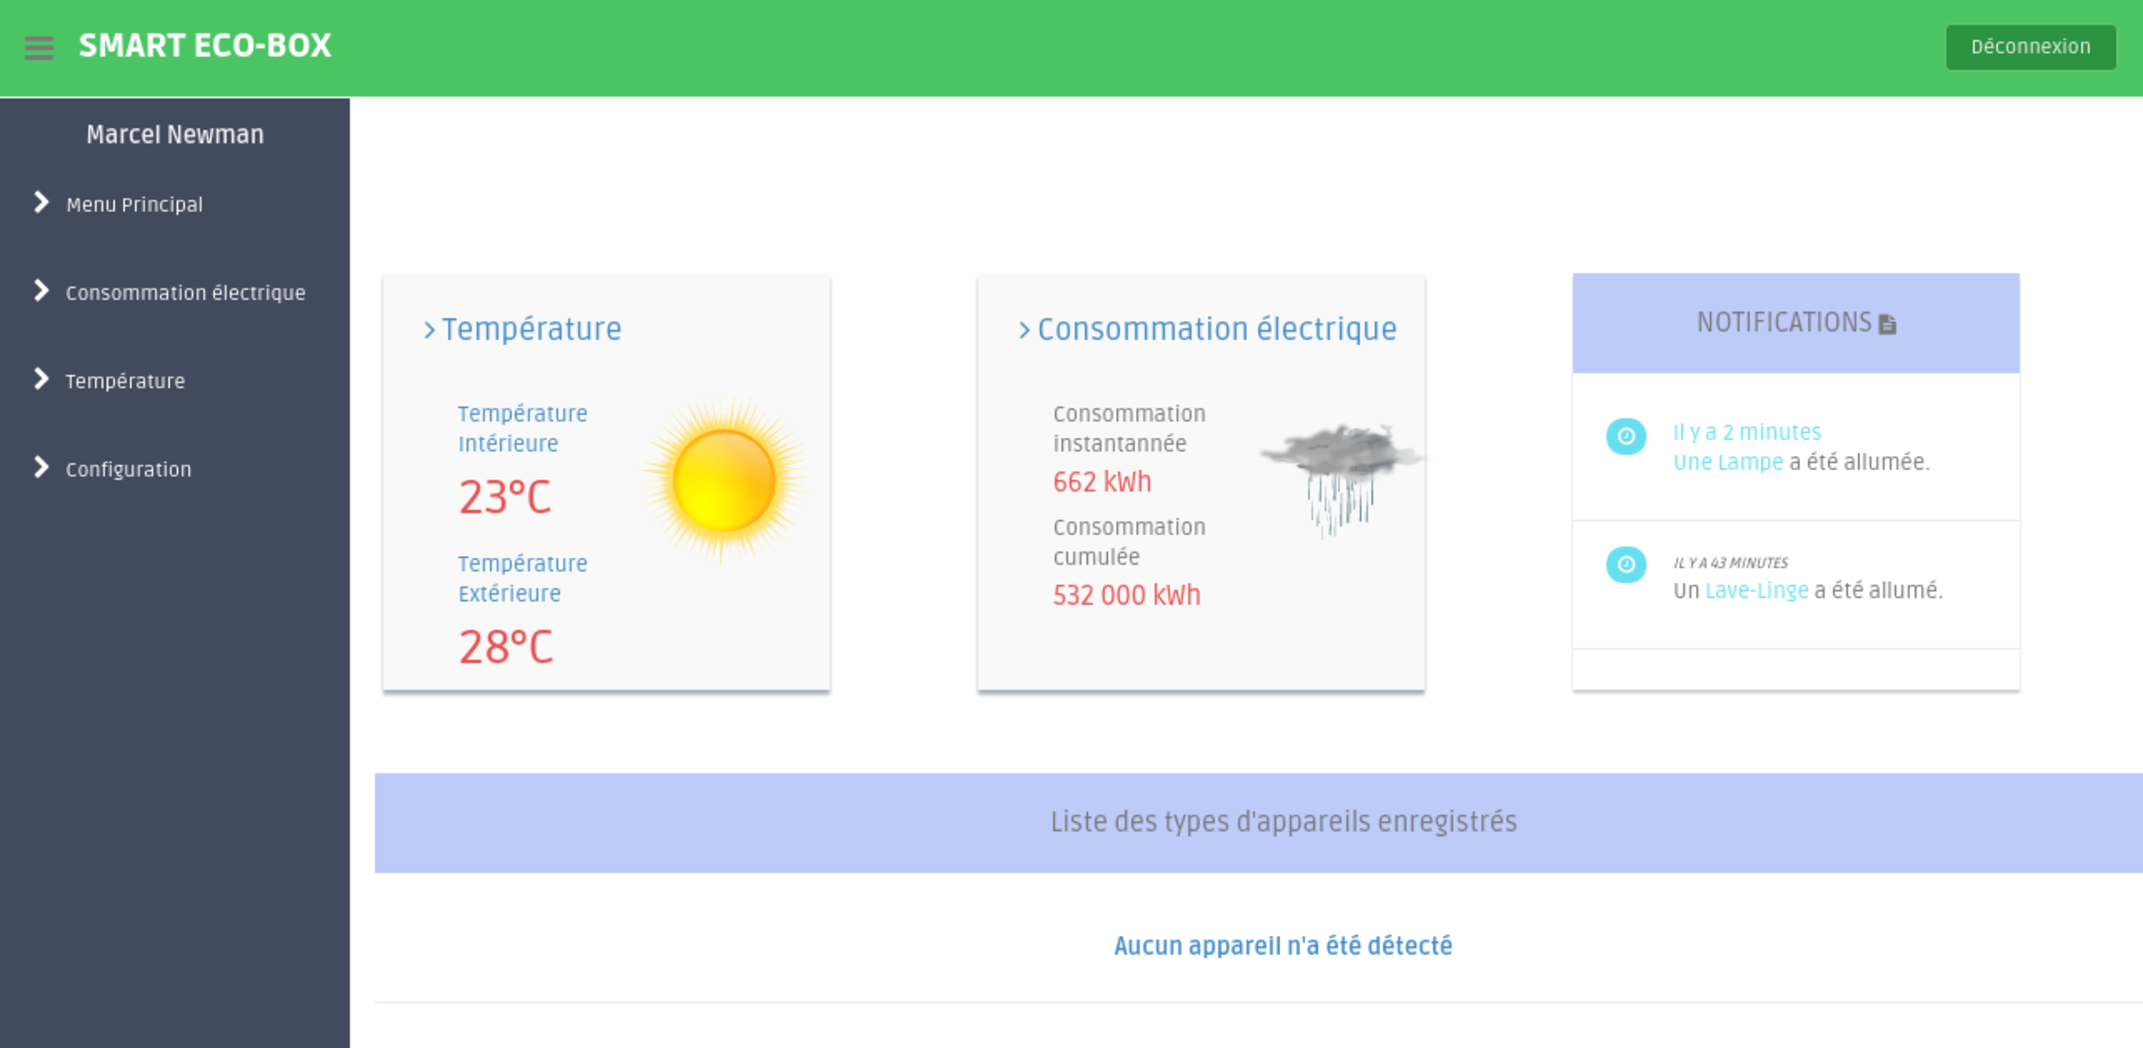
\includegraphics[scale=0.4]{figures/Accueil.pdf}
\caption{Homepage of the webapp}
\label{fig:Accueil}
\end{figure}
This subsection introduces the design of the web interface, especially the structure and the implementation of the main features.
% expliquer l'utilité de l'interface

%%%%%%%%%%%%%%%%%%%%%%%%%%%%%%%%%%%%%%%%%%%%%%%%%%%%%%%%%%%%%%%%%%%%%%%%%%%%%
\subsubsection{Structure}
    % serveur léger -> traitement côté client -> JS -> Angular
    % parler MVC avec Angular
    % n3-chart : n3-chart makes creating beautiful charts for AngularJS application easy and semantic. It is built on top of D3.js library.
    %
    % schéma du site
    Given that the server has to be light and has only to provide the data, this interface has been built with the framework AngularJS 1.3. Indeed, it enables efficient and easily maintainable client-side data processing. In addition, it is based on the Model-View-Controller architectural pattern (MVC) that allows easy maintenance of the code. The curves have been built with the n3-chart library. It makes creating charts for AngularJS application easy and semantic and it is built on top of D3.js library.
    
    The interface has four main pages reachable via the navigation bar: Homepage, Power Consumption page, Temperature page and the Configuration page. Besides, the login page to access the web app and the page to set up and configure the box are designed.
     
    \begin{figure}[!h] 
        \centering
        % pour changer la couleur
        %%  cf main.tex à \tikzstyle pour tout le document
        %   ou
        %%  cf webapp.tex pour savoir comment changer la couleur d'un node
        \begin{tikzpicture}[node distance=1.5cm]
    
        \node (startConf) [startstop] {Setting up and Configuring};
        \node (login) [process, below of=startConf] {Log in};
        \node (home) [process, below of=login] {Homepage};
        \node (conf) [process, below of=home] {Configuration};
        \node (conso) [process, right of=conf, xshift=2cm] {Power Consumption};
        \node (temp) [process, left of=conf, xshift=-2cm] {Temperature};

        \draw [arrow] (startConf) -- (login);
        \draw [arrow] (login) -- (home);
        \draw [arrow] (home) -- (conf);
        \draw [arrow] (home) -- (conso);
        \draw [arrow] (home) -- (temp);
        \end{tikzpicture}
    \end{figure}

     
%%%%%%%%%%%%%%%%%%%%%%%%%%%%%%%%%%%%%%%%%%%%%%%%%%%%%%%%%%%%%%%%%%%%%%%%%%%%%
\subsubsection{Homepage}

The homepage provides quick access to the general state of the system.
The main information related to the system's operation and an overview of the data sent by the sensors can be found on this page.
The homepage includes four main blocks:%, - one for electric consumption and one for temperature, one for notifications and one for the states of registered devices - where the most important data will be indicated.
    \paragraph{Power Consumption} 
    This block provides access to two types of information: the instantaneous and accumulated power consumption. An icon related to the theme of meteorology indicates the evolution of these data. % TODO Button to switch and see the cost
    \paragraph{Temperature}
    This block provides access to two main information: inside and outside temperatures.
    \paragraph{Notifications}
    This block enables the user to monitor changes of sensor statuses and registered types of device statuses. The system notifies the user when a status changes.
    %State sensor
    %State registered devices
    \paragraph{List of Devices} % Liste des types d’appareils enregistrés
    This block provides access to all registered types of devices and their statuses.
    %know the state of all registered type of devices.

%%%%%%%%%%%%%%%%%%%%%%%%%%%%%%%%%%%%%%%%%%%%%%%%%%%%%%%%%%%%%%%%%%%%%%%%%%%%%
\subsubsection{Power Consumption}

    \paragraph{Curve Page}
    % suivre evolution de sa conso
    %   courbe de conso
    %   courbe de coût associé
    %   coût cumulé sur la période.
    The user can access the evolution of his domestic power consumption thanks to three elements of information: the power consumption curve, the matched cost curve and the accumulated cost.
    
    \paragraph{Estimated Electricity Bill}
    An estimated electricity bill can be viewed on this page. It is inspired by a real electricity bill and allows the user to know an estimate depending on his behavior.
%%%%%%%%%%%%%%%%%%%%%%%%%%%%%%%%%%%%%%%%%%%%%%%%%%%%%%%%%%%%%%%%%%%%%%%%%%%%%
\subsubsection{Temperature}
    % suivre evolution de la temperature au sein sa maison
    %   courbes de temperature
    %   plusieurs capteurs
    For each temperature sensor, a temperature curve can be displayed allowing the user to access the evolution of the temperature within the house. 
%%%%%%%%%%%%%%%%%%%%%%%%%%%%%%%%%%%%%%%%%%%%%%%%%%%%%%%%%%%%%%%%%%%%%%%%%%%%%
\subsubsection{Configuration Pages}
    
    \paragraph{Setting up and Configuring} % configuration à l'allumage
    
    When the user turns on his box for the first time, he needs to register by providing his personal data: name, email, password, city and his EDF subscription. Then, the system automatically displays the different sensors detected thanks to the signal processing algorithm. The user has to set up the system by providing the name, the location and the type of each sensor. % (a color-based recognition could be used)
    
    \paragraph{Current Usage} % pendant l'utilisation
    
    \subparagraph{"My Account" Page:} 
    The user can access his personal information and change them. This includes his name, password, email, city and his EDF subscription. Similarly, the profile appears on the homepage.
    
    \subparagraph{"My Sensors" Page:}
    This page is used to list the different sensors. Each sensor can be renamed by the user, may indicate a location specified by the user (e.g. children's room) and also specifies a type of sensor that is recognized by a color code. Besides, the SNR (Signal-to-Noise Ratio) is indicated as the form of bars to show the state of a sensor (like mobile phone signal bars). Finally, users can edit the sensor information using the "Edit" button.
